\documentclass[UTF8,a4paper]{ctexart}
% \pagestyle{empty}
% \documentclass[a4paper]{article}
\usepackage{amssymb}
\usepackage{amsmath}
\usepackage{geometry}
\usepackage{graphicx}
\usepackage{float}
\usepackage{subfigure}
\usepackage{CJK}
\usepackage{caption}


\usepackage{lastpage}
\usepackage{titlesec}   %设置页眉页脚的宏包
\newpagestyle{main}{            
    \sethead{无42 林子恒 2014011054}{DSP --- DTMF}{page \thepage\ of \pageref{LastPage}}  
    %设置页眉
    %\setfoot{左页脚}{中页脚}{右页脚}      %设置页脚,可以在页脚添加 \thepage  显示页数
    \headrule                                      % 添加页眉的下划线
    \footrule                                      % 添加页脚的下划线
}
\pagestyle{main}    %使用该style

\usepackage{times}
\usepackage{fancybox}
\usepackage{xcolor}
\usepackage{listings}
\lstset{breaklines}
\lstset{language=C++}
\lstset{                        %Settings for listings package.
  language=[ANSI]{C++},
         % numbers=left,
         numberstyle=\tiny,
         basicstyle=\small\ttfamily,
         stringstyle=\color{purple},
         keywordstyle=\color{blue}\bfseries,
         commentstyle=\color{olive},
         directivestyle=\color{blue},
         frame=shadowbox,
         showspaces=false,
       %framerule=0pt,
       %backgroundcolor=\color{pink},
         rulesepcolor=\color{red!20!green!20!blue!20},
         tabsize=4,
      %rulesepcolor=\color{brown}
         xleftmargin=3em, xrightmargin=3em, aboveskip=1em
}


\geometry{left=1.5cm, right=1.5cm, top=2cm, bottom=2cm}

  \author{无42 林子恒 2014011054} 
  \title{DSP 2nd Project --- DTMF Detection}
  \date{2016.11.25}

\CTEXsetup[format={\Large\bfseries}]{section}
\renewcommand{\figurename}{Figure}
\renewcommand{\tablename}{Table}

%%%%%%%%%%%%%%%%%%%%%%%%%%%%%%%%%%%%
\begin{document}
  \maketitle
  \thispagestyle{empty}
	See my Github Repository for more infomation:
	
	https://github.com/lzhbrian/DTMF

\tableofcontents

\newpage


%%%%%%%%%%%%%%%%%%%%%%%%%%%%%%%%%%%%
\section{Problem}
要求利用FFT, Goertzel算法,对给定音频文件中的双音多频信号进行检测和识别。

\begin{enumerate}

\item 下载附件包中第一小题的 10 个长度不一的音频文件,利用第一次课程设计 中编写的 FFT 程序对这 10 个文件中的 DTMF 信号进行频谱分析,最后给出 10 个文件 所对应的真实数字。
\item 编写 Goertzel 算法的 C/C++语言程序,完成(1)中的要求。
\item 下载附件包中第二小题的一个长音频文件,文件中包含了一串 DTMF 信号, 每个双音多频信号之间的时间间隔不一,对本串 DTMF 信号进行识别。

\end{enumerate}


%%%%%%%%%%%%%%%%%%%%%%%%%%%%%%%%%%%%
\section{Solution}


\subsection{Read the .wav files --- read\_wav.m}

We use a Matlab audioread() function to convert the .wav file to .txt file, extracting the time-zone signals. Saving .txt files to ./txtData1 and ./txtData2.

The code is shown in section~\ref{code:readwav}


%!TEX root = dsp_2nd_program_hw.tex

\subsection{Realization of DTMF using FFT --- dif\_fft.h}
This part is explained in the previous report. 
The code is shown in section~\ref{code:fft}

See https://github.com/lzhbrian/Fast-Fourier-Transform for more information. 

\subsection{Realization of DTMF using Goertzel --- goertzel.h}
Goertzel algorithm is a method by which we can only calculate the amplitude of certain frequency.
By the following functions, We can obtain the $X[k]$ we want:
\begin{equation}\label{equation:iter}
v_{k}[n] = x[n] + 2cos(\omega_{k})v_{k}[n-1]-v_{k}[n-2]
\end{equation}
\begin{equation}\label{equation:xk_calc}
X[k] = v_{k}[N-1] - W^{k}_{N}v_{k}[N-2]
\end{equation}
where 
$$\omega_{k} = 2\pi k/N, W_{N}=e^{2\pi /N}, v_{k}[-2]=v_{k}[-1]=0, v_{k}[0]=x[0]$$

In this DTMF detection, we want to acquire the amplitude of 
$$697Hz, 770Hz, 852Hz, 941Hz, 1209Hz, 1336Hz, 1477Hz, 1633Hz$$
Note that we get the $k$ for each frequency by the following equation:
\begin{equation}
k = ( N * f ) / SamplingRate;
\end{equation}
where $N$ is the length of the sequence, and f is the targeted frequency.

So we first iteratively calculate the value of $v_{k}[N-1]$ and $v_{k}[N-2]$ using equation~(\ref{equation:iter}), then we use them to get the value of X[k] by equation~(\ref{equation:xk_calc}).
In the real practice, we further return the amplitude of X[k] by calculating their sum of squares.

The code is shown in section~\ref{code:goertzel}

%!TEX root = dsp_2nd_program_hw.tex
\subsection{DTMF Detection --- find\_dtmf\_symbol.h}
For convenience, we wrote a function to obtain the symbol of a DTMF signal.
By inputing the max two frequency, we can get the symbol $1,2,3,4,5,6,7,8,9,A,B,C,D,0,*,\#$

The code is shown in section~\ref{code:finddtmf}


\subsection{Recognition of Dataset 1 --- 10 signals}
	
\subsubsection{FFT --- DTMF\_1.cpp}
The result is 
$$5,1,6,9,8,7,3,4,0,2$$
for data
$$1081,1107,1140,1219,1234,1489,1507,1611,1942,1944$$
respectively, as shown in Table~\ref{tab:result}.
The code is shown in section~\ref{dtmf1}.

\begin{table}[htp]
\centering
{\small
\begin{tabular}{c|ccc}
    \hline
    \textbf{Signal length} & \textbf{1st freq} & \textbf{2nd freq} & \textbf{symbol} \\ 
    \hline
	   1081 & 769 & 1337 & 5 \\
	   1107 & 696 & 1212 & 1 \\
	   1140 & 770 & 1477 & 6 \\
	   1219 & 852 & 1477 & 9 \\
	   1234 & 852 & 1337 & 8 \\
	   1489 & 852 & 1212 & 7 \\
	   1507 & 696 & 1477 & 3 \\
	   1611 & 770 & 1212 & 4 \\
	   1942 & 942 & 1337 & 0 \\
	   1944 & 696 & 1337 & 2 \\
	\hline
\end{tabular}
}
\vspace{-0.1in}
\caption{DTMF result for 10 respective signals}
\label{tab:result}
\end{table}

\subsubsection{Goertzel --- DTMF\_2.cpp}
Goertzel has shown exactly same result with FFT. The code is shown in section~\ref{dtmf2}.








\newpage

\subsection{Recognition of Dataset 2 --- A long signal, DTMF\_3.cpp}

\subsubsection{Judge the start-end time}
By Matlab, we can obtain the time-zone signals as shown in Figure~\ref{fig:timezone3}. We then manually get the start, end time of each of signal as shown in Table~\ref{tab:startendtime}.
\begin{figure}[htp]
	\centering
	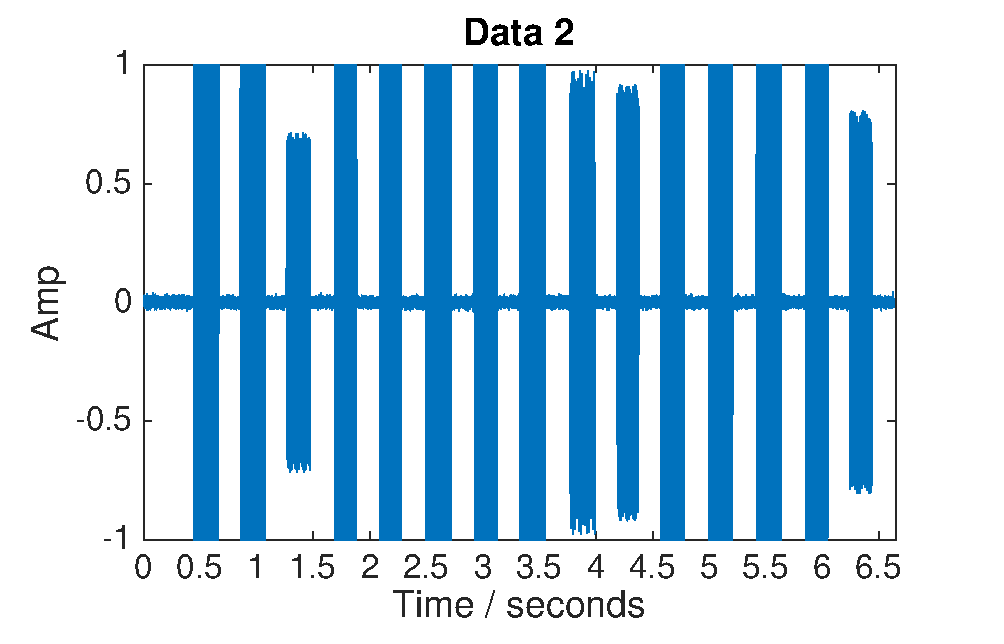
\includegraphics[width=10cm]{../fig/data2.eps}
	\vspace{-0.1in}
	\caption{Timezone signal of Data 2}
	\label{fig:timezone3}

\end{figure}
\vspace{-0.2in}

\begin{table}[htp]
\centering
{\small
\begin{tabular}{c|cc|c|cc}
    \hline
    \textbf{\#} & \textbf{Start time} & \textbf{End time} & \textbf{\#} & \textbf{Start time} & \textbf{End time} \\ 
    \hline
	   1 & 0.45 & 0.66	& 9   & 3.78 & 4.00	\\
	   2 & 0.86 & 1.07	& 10  & 4.18 & 4.40	\\
	   3 & 1.27 & 1.47	& 11  & 4.58 & 4.79	\\
	   4 & 1.70 & 1.89	& 12  & 5.01 & 5.22	\\
	   5 & 2.09 & 2.29	& 13  & 5.43 & 5.64	\\
	   6 & 2.50 & 2.72	& 14  & 5.87 & 6.06	\\
	   7 & 2.92 & 3.10	& 15  & 6.26 & 6.45	\\
	   8 & 3.34 & 3.55	& & &\\
	\hline
\end{tabular}
}
\vspace{-0.1in}
\caption{Start-End time of each signal}
\label{tab:startendtime}
\end{table}
\vspace{-0.3in}

\subsubsection{Result}
By the Goertzel method, we can obtain the symbols for the long signal are:
$$2,0,5,8,9,1,1,3,2,0,u,4,6,4,9$$
$u$ represents unknown, i.e. we cannot detect the 11th symbol, its amplitude response is shown in Figure~\ref{fig:freq11}.From the figure, we can see that we don't have two target frequencies which have a significant amplitude, s.t. we cannot decipher this symbol. The code is shown in section~\ref{dtmf3}.
\begin{figure}[htp]
	\centering
	\includegraphics[width=16cm]{../fig/freq_11.png}
	\caption{Amplitude response of the 11th symbol}
	\label{fig:freq11}
\end{figure}







\newpage

%!TEX root = dsp_2nd_program_hw.tex

\section{Code}


\subsection{DTMF\_1.cpp --- Main function for problem 1}\label{dtmf1}
\begin{lstlisting}
// Work by Lin, Tzu-Heng
// W42, 2014011054
// Dept. of Electronic Engineering, Tsinghua University
// DSP Course Work

# include <fstream>
# include <string>
# include <stdio.h>
# include <stdlib.h>
# include <cmath>
# include <ctime>
# include <sstream>
# include <iostream>
# include <cstdlib>
# include <unistd.h>  
# include <dirent.h>  
# include <sys/stat.h>  
# define PI 3.1415926
int const MAX_STR_LEN = 200;  

# include "complex.h"
# include "dif_fft.h"
# include "find_dtmf_symbol.h"

using namespace std;

// FFT Algorithm
int main()
{
	char dir_name[100] = "./txtData1/"; 

    struct dirent * filename;    // return value for readdir()  
    DIR * dir;                   // return value for opendir()  
    dir = opendir( dir_name );  
    /* read all the files in the dir ~ */  
    while( ( filename = readdir(dir) ) != NULL )  
    {  
        // get rid of "." and ".."  
        if( strcmp( filename->d_name , "." ) == 0 ||   
            strcmp( filename->d_name , "..") == 0 )  
            continue;  
        cout << filename ->d_name <<endl;  
    
    	char hhh[MAX_STR_LEN];
    	strcpy(hhh, dir_name);
    	strcat(hhh, (filename->d_name));
		ifstream in( hhh );
		string filename;
		string line;
		
		if(in) // 有该文件  
		{
			double audio[60000];
			int count = 0;
			while (getline (in, line)) // line中不包括每行的换行符
			{
				// audio[count] = atof(const_cast<const char *>(line.c_str()));

				double d;
				stringstream ss(line);
				ss >> d;
				audio[count] = d;

				count = count + 1;
				// cout << audio[count-1] << endl;
			}

			// is 2^k or not, if not add zero
			int add_zero_count = 0;
			for (int i = 1; i < 100; ++i)
			{
				if ( pow(2,i) < count ) {
					continue;
				} else if ( pow(2,i) == count ) {
					break;
				} else {
					add_zero_count = pow(2,i) - count;
					break;
				}
			}

			// add value to input_seq[]
			int total_length = count + add_zero_count;
			complex* input_seq = new complex[total_length];
			for (int i = 0; i < count; i++)
			{
				input_seq[i].re = audio[i];
				input_seq[i].im = 0;
			}
			for (int i = 0; i < add_zero_count; i++)
			{
				input_seq[count + i].re = 0;
				input_seq[count + i].im = 0;
			}

			// FFT
			complex* output_seq = DIF_FFT_reordered(input_seq, total_length);

			// Amp, Find max 1,2 and their positions
			int amp;
			int max1 = 0;
			int max2 = 0;
			int max1_pos = 0;
			int max2_pos = 0;
			for (int i = 0; i < total_length/2; ++i)
			{
				amp = pow(output_seq[i].re,2) + pow(output_seq[i].im,2);
				if (amp > max2)
				{
					if (amp > max1) {
						// max2 = max1
						max2 = max1;
						max2_pos = max1_pos;
						// max1 = new
						max1 = amp;
						max1_pos = i;
					} else {
						max2 = amp;
						max2_pos = i;
					}
				}
			}

			// x-axis
				// 0:f_s/(N-1):f_s
			int fs = 8000;
			int N = total_length;
			double step = double(fs)/(N-1);
			double* x_axis = new double[N];
			for (int i = 0; i < N; ++i)
			{
				x_axis[i] = i * step;
			}

			// Get max1, max2 freq
			cout << "Max1 pos:" << x_axis[max1_pos] << endl;
			cout << "Max2 pos:" << x_axis[max2_pos] << endl;

			// decipher
			char output_symbol = find_dtmf_symbol(x_axis[max1_pos], x_axis[max2_pos]);
			cout << "The symbol for this sound: " << output_symbol << endl;

			cout << endl;

		} else { // fail reading file
			cout << "no such file" << endl;
		}
    }  
	return 0;
}
\end{lstlisting}

\subsection{DTMF\_2.cpp --- Main function for problem 2}\label{dtmf2}
\begin{lstlisting}
// Work by Lin, Tzu-Heng
// W42, 2014011054
// Dept. of Electronic Engineering, Tsinghua University
// DSP Course Work

# include <fstream>
# include <string>
# include <stdio.h>
# include <stdlib.h>
# include <cmath>
# include <ctime>
# include <sstream>
# include <iostream>
# include <cstdlib>
# include <unistd.h>  
# include <dirent.h>  
# include <sys/stat.h>  
# define PI 3.1415926
int const MAX_STR_LEN = 200;  

# include "complex.h"
# include "goertzel.h"
# include "find_dtmf_symbol.h"

using namespace std;

// Goertzel Algorithm
int main()
{
	cout << "Running Prob2, using Goertzel Algorithm ... " << endl << endl;

	char dir_name[100] = "./txtData1/"; 

    struct dirent * filename;    // return value for readdir()  
    DIR * dir;                   // return value for opendir()  
    dir = opendir( dir_name );  
    /* read all the files in the dir ~ */  
    while( ( filename = readdir(dir) ) != NULL )  
    {  
        // get rid of "." and ".."  
        if( strcmp( filename->d_name , "." ) == 0 ||   
            strcmp( filename->d_name , "..") == 0 )  
            continue;  
        cout << filename ->d_name <<endl;  
    
    	char hhh[MAX_STR_LEN];
    	strcpy(hhh, dir_name);
    	strcat(hhh, (filename->d_name));
		ifstream in( hhh );
		string filename;
		string line;
		
		if(in) // 有该文件  
		{
			double audio[60000];
			int count = 0;
			while (getline (in, line)) // line中不包括每行的换行符
			{
				// audio[count] = atof(const_cast<const char *>(line.c_str()));

				double d;
				stringstream ss(line);
				ss >> d;
				audio[count] = d;

				count = count + 1;
				// cout << audio[count-1] << endl;
			}

			// is 2^k or not, if not add zero
			int add_zero_count = 0;
			for (int i = 1; i < 100; ++i)
			{
				if ( pow(2,i) < count ) {
					continue;
				} else if ( pow(2,i) == count ) {
					break;
				} else {
					add_zero_count = pow(2,i) - count;
					break;
				}
			}

			// add value to input_seq[]
			int total_length = count + add_zero_count;
			complex* input_seq = new complex[total_length];
			for (int i = 0; i < count; i++)
			{
				input_seq[i].re = audio[i];
				input_seq[i].im = 0;
			}
			for (int i = 0; i < add_zero_count; i++)
			{
				input_seq[count + i].re = 0;
				input_seq[count + i].im = 0;
			}

			// Goertzel, return amp^2
			double* targeted_amp = Goertzel(input_seq, total_length);

			// Amp, Find max 1,2 and their positions
			int amp;
			int max1 = 0;
			int max2 = 0;
			int max1_pos = 0;
			int max2_pos = 0;
			for (int i = 0; i < 8; ++i)
			{
				amp = targeted_amp[i];
				if (amp > max2)
				{
					if (amp > max1) {
						// max2 = max1
						max2 = max1;
						max2_pos = max1_pos;
						// max1 = new
						max1 = amp;
						max1_pos = i;
					} else {
						max2 = amp;
						max2_pos = i;
					}
				}
			}

			// Get max1, max2 freq
			double x_axis[] = 				 		{697,
											  		 770,
											  		 852,
											  		 941,
								1209,1336,1477,1633};

			cout << "Max1 pos:" << x_axis[max1_pos] << endl;
			cout << "Max2 pos:" << x_axis[max2_pos] << endl;

			// decipher
			char output_symbol = find_dtmf_symbol(x_axis[max1_pos], x_axis[max2_pos]);
			cout << "The symbol for this sound: " << output_symbol << endl;

			cout << endl;

		} else { // fail reading file
			cout << "no such file" << endl;
		}

    }  
	return 0;
}
\end{lstlisting}

\subsection{DTMF\_3.cpp --- Main function for problem 3}\label{dtmf3}
\begin{lstlisting}
// Work by Lin, Tzu-Heng
// W42, 2014011054
// Dept. of Electronic Engineering, Tsinghua University
// DSP Course Work

# include <fstream>
# include <string>
# include <stdio.h>
# include <stdlib.h>
# include <cmath>
# include <ctime>
# include <sstream>
# include <iostream>
# include <cstdlib>
# include <unistd.h>  
# include <dirent.h>  
# include <sys/stat.h>  
# define PI 3.1415926
int const MAX_STR_LEN = 200;  

# include "complex.h"
# include "goertzel.h"
# include "find_dtmf_symbol.h"

using namespace std;

// Goertzel Algorithm to identify 3
int main()
{

		cout << "Identifying Prob3, a long audio, using Goertzel Algorithm ..." << endl << endl;

		ifstream in("./txtData2/data.txt");
		string filename;
		string line;
		
		if(in) // 有该文件  
		{
			double audio[60000];
			int count = 0;
			while (getline (in, line)) // line中不包括每行的换行符
			{
				// audio[count] = atof(const_cast<const char *>(line.c_str()));

				double d;
				stringstream ss(line);
				ss >> d;
				audio[count] = d;

				count = count + 1;
				// cout << audio[count-1] << endl;
			}

			// Stops (in seconds)
			double stops[] = 	{0.4459, 0.6633,
							     0.8642, 1.072,
							     1.27,   1.473,
							     1.7,    1.89,
							     2.09,   2.29,
							     2.5,    2.722,
							     2.915,  3.1,
							     3.34,   3.549,
							     3.782,  4,
							     4.182,  4.398, 
							     4.581,  4.794,
							     5.013,  5.222, 
							     5.431,  5.641, 
							     5.869,  6.059, 
							     6.258,  6.447};

		    int len_data2 = count;
			double seconds_len_data2 = len_data2/8000.0;

			for (int d = 0; d < 15; ++d)
			{

				int start_index = stops[d*2]/seconds_len_data2*len_data2;
				int end_index = stops[d*2+1]/seconds_len_data2*len_data2;

				// Get this audio
				count = end_index - start_index + 1;
				double* this_audio = new double[count];
				for (int i = 0; i < count; ++i)
				{
					this_audio[i] = audio[i+start_index];
				}

				// is 2^k or not, if not add zero
				int add_zero_count = 0;
				for (int i = 1; i < 100; ++i)
				{
					if ( pow(2,i) < count ) {
						continue;
					} else if ( pow(2,i) == count ) {
						break;
					} else {
						add_zero_count = pow(2,i) - count;
						break;
					}
				}

				// add value to input_seq[]
				int total_length = count + add_zero_count;
				complex* input_seq = new complex[total_length];
				for (int i = 0; i < count; i++)
				{
					input_seq[i].re = this_audio[i];
					input_seq[i].im = 0;
				}
				for (int i = 0; i < add_zero_count; i++)
				{
					input_seq[count + i].re = 0;
					input_seq[count + i].im = 0;
				}

				// Goertzel, return amp^2
				double* targeted_amp = Goertzel(input_seq, total_length);

				// amp indicator
				// for (int ii = 0; ii < 8; ++ii)
				// {
				// 	cout << targeted_amp[ii] << endl;
				// }

				// Amp, Find max 1,2 and their positions
				int amp;
				int max1 = 0;
				int max2 = 0;
				int max1_pos = 0;
				int max2_pos = 0;
				for (int i = 0; i < 8; ++i)
				{
					amp = targeted_amp[i];
					if (amp > max2)
					{
						if (amp > max1) {
							// max2 = max1
							max2 = max1;
							max2_pos = max1_pos;
							// max1 = new
							max1 = amp;
							max1_pos = i;
						} else {
							max2 = amp;
							max2_pos = i;
						}
					}
				}

				// Get max1, max2 freq
				double x_axis[] = 				 		{697,
												  		 770,
												  		 852,
												  		 941,
									1209,1336,1477,1633};

				cout << "Max1 pos:" << x_axis[max1_pos] << endl;
				cout << "Max2 pos:" << x_axis[max2_pos] << endl;

				// decipher
				char output_symbol = find_dtmf_symbol(x_axis[max1_pos], x_axis[max2_pos]);
				cout << "The symbol for this sound: " << output_symbol << endl;

				cout << endl;

			}

		} else { // fail reading file
			cout << "no such file" << endl;
		}
	

	return 0;
}
\end{lstlisting}


\subsection{complex.h}\label{code:complex}
\begin{lstlisting}
// Work by Lin, Tzu-Heng
// W42, 2014011054
// Dept. of Electronic Engineering, Tsinghua University
// DSP Course Work

/********************************************************************/
// Complex Struct & Some Basic func


using namespace std;

typedef struct Complex
{
	double re;
	double im;
	Complex() {
		re = 0;
		im = 0;
	};
	Complex(double a,double b) {
		re = a;
		im = b;
	};
} complex;


complex* append_seq(complex seq_1[], complex seq_2[], int N);
complex* reorder_seq(complex input_seq[], int N);
complex* Calc_WN(int N);
int reverse_bit(int value, int N);

// Multiplier
complex ComplexMul(complex c1, complex c2)
{
	complex r;
	
	r.re = c1.re*c2.re - c1.im*c2.im;
	r.im = c1.re*c2.im + c1.im*c2.re;

	return r;
}

// Adder
complex ComplexAdd(complex c1, complex c2)
{
	complex r;
	
	r.re = c1.re + c2.re;
	r.im = c1.im + c2.im;
	
	return r;
}

// -c
complex ReverseComplex(complex c)
{
	c.re = -c.re;
	c.im = -c.im;
	
	return c;
}

// scalar mul
complex ComplexScalarMul(complex cc, double con)
{
	complex r;
	
	r.re = cc.re * con;
	r.im = cc.im * con;

	return r;
}

// Other func


/********************************************************************/
// Append [seq_1] & [seq_2] to [seq_1,seq_2]
complex* append_seq(complex seq_1[], complex seq_2[], int N) {
	complex* total_seq = new complex[N*2];
	for (int i = 0; i < N; i++) {
		total_seq[i] = seq_1[i];
	}
	for (int i = N; i < 2*N; i++) {
		total_seq[i] = seq_2[i-N];
	}
	return total_seq;
}


/********************************************************************/
// Reorder the input_seq to an order
complex* reorder_seq(complex input_seq[], int N) {

	cout << "Reorder the sequence ..." << endl;

	complex* reordered_seq = new complex[N];
	for (int i = 0; i < N; ++i)
	{
		int k = reverse_bit(i, log2(N));
		reordered_seq[k] = input_seq[i];
	}

	return reordered_seq;
}


/********************************************************************/
// Reverse Bit
	// input: 
		// a decimal num, 
		// N-based reverse method
	// output: a decimal num
int reverse_bit(int value, int N) {

	int ret = 0;
	int i = 0;

	while (i < N) {
		ret <<= 1;
		ret |= (value>>i) & 1;
		i++;
	}

	return ret;
}


/********************************************************************/
// Calc WN[], with N = input_N
complex* Calc_WN(int N) {

	cout << "Calculating WN[] of N = " << N << " ..." << endl;
	complex* WN = new complex[N];

	complex WN_unit; WN_unit.re = cos(2*PI/N); WN_unit.im = -sin(2*PI/N);
	WN[0].re=1; WN[0].im=0;

	for (int i = 1; i < N; ++i)
	{
		WN[i] = ComplexMul(WN[i-1], WN_unit);
	}

	return WN;
}
\end{lstlisting}

\subsection{dif\_fft.h --- FFT implementation}\label{code:fft}
\begin{lstlisting}
// Work by Lin, Tzu-Heng
// W42, 2014011054
// Dept. of Electronic Engineering, Tsinghua University
// DSP Course Work

complex* DIF_FFT_reordered(complex input_seq[], int N);
complex* DIF_FFT(complex input_seq[], int N, complex WN[], int recur_time_count);

/********************************************************************/
// DIF-FFT
	// input_seq[]: 
	// N: size of input_seq
		// Must be a 2^k integer
complex* DIF_FFT_reordered(complex input_seq[], int N) {
	
	// Initialize
	complex* reordered_seq = new complex[N];
	
	// Calc WN
	complex* WN = new complex[N];
	WN = Calc_WN(N);

	// Calc DIF-FFT
	reordered_seq = DIF_FFT(input_seq, N, WN, 0);
	// Reorder
	reordered_seq = reorder_seq(reordered_seq, N);

	return reordered_seq;
}
complex* DIF_FFT(complex input_seq[], int N, complex WN[], int recur_time_count) {

	// cout << "\tDIF_FFT executed!\n"; // for validation
	// output seq
	complex* return_seq = new complex[N];

	if ( N != 2 ) {

		complex* first_half_seq = new complex[N/2];
		complex* second_half_seq = new complex[N/2];

		int k = pow(2,recur_time_count);

		// Calc
		for (int i = 0; i < N/2; ++i) {
			first_half_seq[i] = ComplexAdd(input_seq[i], input_seq[i+N/2]) ;
		}
		for (int i = 0; i < N/2; ++i) {
			second_half_seq[i] = ComplexMul( ComplexAdd(input_seq[i], ReverseComplex(input_seq[i+N/2])), WN[i*k] ) ;
		}

		// DFT
		complex* DFTed_first_half_seq = new complex[N/2];
		DFTed_first_half_seq = DIF_FFT(first_half_seq, N/2, WN, recur_time_count+1);
		complex* DFTed_second_half_seq = new complex[N/2];
		DFTed_second_half_seq = DIF_FFT(second_half_seq, N/2, WN, recur_time_count+1);

		// Append [DFTed_first_half_seq] & [DFTed_second_half_seq]
		return_seq = append_seq(DFTed_first_half_seq, DFTed_second_half_seq, N/2);
		return return_seq;

	} else if ( N == 2 ) { // Smallest Butterfly Unit

		// cout << "\tDIF_FFT N==2 triggered!\n"; // for validation
		return_seq[0] = ComplexAdd(input_seq[0], input_seq[1]);
		return_seq[1] = ComplexMul( ComplexAdd(input_seq[0], ReverseComplex(input_seq[1])), WN[0] );
		return return_seq;
	
	}

	// return [return_seq] # unordered
	return return_seq;
}
/********************************************************************/
\end{lstlisting}


\subsection{goertzel.h --- Goertzel implementation}\label{code:goertzel}
\begin{lstlisting}
// Work by Lin, Tzu-Heng
// W42, 2014011054
// Dept. of Electronic Engineering, Tsinghua University
// DSP Course Work

// input x[n], N
// output: amp of the targeted 8 freq (freqs)

double* Goertzel(complex input_seq[], int N) {

	cout << "Calculating Goertzel ..." << endl;
	// targeted freqs
	double freqs[] = 				 		{697,
									  		 770,
									  		 852,
									  		 941,
						1209,1336,1477,1633};

	// Calc WN
	complex* WN = new complex[N];
	WN = Calc_WN(N);

	int sampling_rate = 8000;

	// Calc DFT of targeted 8 freqs
	complex targeted_X[8];
	complex* v = new complex[N];

	for (int i = 0; i < 8; ++i)
	{	
		int k = ( N * freqs[i] ) / sampling_rate;
		double w_k = 2 * PI * k / N;

		// init
		v[0] = input_seq[0];
		v[1] = ComplexAdd(input_seq[1], ComplexScalarMul(v[0], 2*cos(w_k)));

		for (int j = 2; j < N; ++j)
		{
			v[j] = ComplexAdd(ComplexAdd(input_seq[j], ComplexScalarMul(v[j-1], 2*cos(w_k))), ReverseComplex(v[j-2]));
		}

		targeted_X[i] = ComplexAdd(v[N-1], ReverseComplex(ComplexMul(WN[k], v[N-2])));
	}

	// Calc amp
	double* amp_targeted_X = new double[8];
	for (int i = 0; i < 8; ++i)
	{
		amp_targeted_X[i] = pow(targeted_X[i].re,2) + pow(targeted_X[i].im,2);
		// cout << amp_targeted_X[i] << endl; // indicator
	}

	return amp_targeted_X; 
}
\end{lstlisting}


\subsection{find\_dtmf\_symbol.h --- judge signals}\label{code:finddtmf}
\begin{lstlisting}
// Work by Lin, Tzu-Heng
// W42, 2014011054
// Dept. of Electronic Engineering, Tsinghua University
// DSP Course Work

// Decipher
char find_dtmf_symbol(double a, double b)
{
	char symbol[]	 =  {'1','2','3','A',
						 '4','5','6','B',
						 '7','8','9','C',
						 '*','0','#','D'};
	double freqs1[] = 				 		{697,
									  		 770,
									  		 852,
									  		 941};
	double freqs2[] = {1209,1336,1477,1633};

	// switch if a > b, making sure a < b
	if (a > b) {
		int c = a;
		a = b;
		b = c;
	}

	// get a pos: x
	int x = 100;
	for (int i = 0; i < 4; ++i)
	{
		if ( abs(freqs1[i] - a) <= 10 )
		{
			x = i;
			break;
		}
	}

	// get b pos: y
	int y = 100;
	for (int i = 0; i < 4; ++i)
	{
		if ( abs(freqs2[i] - b) <= 10 )
		{
			y = i;
			break;
		}
	}

	if (x == 100 || y == 100)
	{
		char error_char = 'x';
		return error_char;
	}
	// get return symbol
	char return_symbol = symbol[ x*4 + y ];

	return return_symbol;
}
\end{lstlisting}



\subsection{read\_wav.m --- Convert .wav files to .txt}\label{code:readwav}
\begin{lstlisting}
// Work by Lin, Tzu-Heng
// W42, 2014011054
// Dept. of Electronic Engineering, Tsinghua University
// DSP Course Work

close all;clc;clear;

%% Data1
dirpath = './Data1/';
writepath = './txtData1/';
dat = dir( dirpath );
for j = 1 : length( dat )
    if( ~isequal( dat( j ).name, '.' ) &...
        ~isequal( dat( j ).name, '..') )
        datpath = [dirpath dat( j ).name];
        [y, Fs] = audioread(datpath);
        f = fopen([writepath dat( j ).name(1:8) '.txt'],'w');
        fprintf(f, '%f\n', y);
        fclose(f);
    end
end

%% Data2
datpath = './Data2/data.wav';
[y, Fs] = audioread(datpath);
f = fopen('./txtData2/data.txt','w');
fprintf(f, '%f\n', y);
fclose(f);
\end{lstlisting}



\end{document}








